\documentclass[matan]{subfiles}

\begin{document}
  \newpage
  \section{Асимптотика частичных сумм расходящегося ряда (случай гармонического ряда). Постоянная Эйлера.}

  \[\frac{1}{1+k} = \frac{\frac{1}{k}}{\frac{1}{k}+1} < \ln(1+\frac{1}{k}) < \frac{1}{k} \Rightarrow 0 < \frac{1}{k} - \ln(1+\frac{1}{k})< \frac{1}{k}-\frac{1}{k+1}\]

  Значит, \begin{multline*}
      $$0 < \sum\limits_{k=1}^n \big(\dfrac{1}{k} - \ln(1+\dfrac{1}{k})\big) < \sum\limits_{k=1}^n \big(\dfrac{1}{k} - \dfrac{1}{k+1}\big) = \\
      =1 - \cancel{\frac{1}{2}} + \cancel{\frac{1}{2}} - \cancel{\frac{1}{3}} + \cancel{\frac{1}{3}} -...+ \cancel{\frac{1}{n}} - \frac{1}{n-1} =\\
      =1 - \frac{1}{n+1} = \frac{n}{n+1} < 1\ \forall n \in \N$$
  \end{multline*}
  \\
  $\Rightarrow S_n := \sum\limits_{k=1}^n \big(\dfrac{1}{k} - \ln(1+\dfrac{1}{k})\big) \nearrow$ и ограничено сверху $\Rightarrow \e \lim\limits_{n \rightarrow \infty} S_n$

  $$\sum\limits_{k=1}^n \ln (1+ \frac{1}{k}) = \sum\limits_{k=1}^n (\ln(k+1) - \ln(k)) = -\ln1+\cancel{\ln2}-\cancel{\ln2}+\cancel{\ln3}-...-\cancel{\ln (n)}+ \ln (n+1) =$$
  $$ =\ln (n+1) \Rightarrow \e \lim\limits_{n \rightarrow \infty} \sum\limits_{k=1}^n \frac{1}{k} - \ln (n+1) = \lim\limits_{n \rightarrow \infty} (\sum\limits_{k=1}^n \frac{1}{k} - \ln n)$$

  \begin{definition}
      $\upgamma := \lim\limits_{n \rightarrow \infty} (\sum\limits_{k=1}^n \dfrac{1}{k} - \ln n) = 0,5722...$ - постоянная Эйлера
  \end{definition}

  \newpage
  \section{Несобственные интегралы. Примеры. Несобственный интеграл в смысле главного значения. Критерий Больцано-Коши для несобственных интегралов.}

  \begin{definition}[1]
      $f: [a, +\infty) \rightarrow \R$, $f \in R[a,b]$ $\forall b \in (a, +\infty).$
      \begin{multline*}
          $$\text{Если }\e \lim\limits_{b \rightarrow \infty} \int\limits_a^b f, \text{ то говорят, что несобственный интеграл} \\
          \int\limits_a^{+\infty} f \text{ - сходится и равен } \lim\limits_{b \rightarrow \infty} \int\limits_a^b f$$
      \end{multline*}
  \end{definition}

  \begin{definition}[2]
      $f: [a, \upomega) \rightarrow \R$, $-\infty < a < \upomega \leqslant +\infty$ ,\ $f \in R[a,b]$ $\forall b \in (a, +\infty)$.
      \begin{multline*}
          $$\text{Если }\e \lim\limits_{b \rightarrow \upomega_-} \int\limits_a^b f,\text{ то говорят, что несобственный интеграл } \\
          \int\limits_a^{\upomega} f\text{ - сх и равен } \lim\limits_{b \rightarrow \upomega_-} \int\limits_a^b f$$
      \end{multline*}
  \end{definition}

  \begin{definition}[3]
      $f: \R \rightarrow \R$ и $\forall a<b\in \R: f \in R[a,b]$, тогда $\int\limits_{-\infty}^{+\infty} f := \lim\limits_{a \rightarrow -\infty} \int\limits_a^0 f + \lim\limits_{b \rightarrow +\infty} \int\limits_0^b f$,

      Если оба предела $\e$ и конечны, то говорят что $\int\limits_{-\infty}^{+\infty} f$ - сходится
  \end{definition}

  \begin{definition}[4]
      Аналогично $\int\limits_{\upomega_1}^{\upomega_2}$, если $f \in R[a,b]$ $\forall[a,b] \subset (\upomega_1,\upomega_2)$. $\int\limits_{\upomega_1}^{\upomega_2} f= \int\limits_{\upomega_1}^c f + \int\limits_c^{\upomega_2}$
  \end{definition}

  \begin{example}
      \begin{enumerate}
          \item $\upalpha = 1$, $\int\limits_1^{+\infty} \dfrac{dx}{x^\upalpha} = \lim\limits_{b \rightarrow +\infty} \ln |x| \big|_1^b = +\infty$ - расх
          \item $\upalpha > 1$, $\int\limits_1^{+\infty} \dfrac{dx}{x^\upalpha} = \lim\limits_{b \rightarrow +\infty} \dfrac{x^{1-\upalpha}}{1-\upalpha} \Big|_1^b = 0-\dfrac{1}{1-\upalpha}$ - сх
          \item $\upalpha < 1$, $\int\limits_1^{+\infty} \dfrac{dx}{x^\upalpha} =  +\infty$ - расх
      \end{enumerate}
  \end{example}

  \begin{Example}
      \[\int\limits_{-1}^1 \frac{dx}{x} = \lim\limits_{a \rightarrow 0_-} \int\limits_{-1}^a \frac{dx}{x} + \lim\limits_{b \rightarrow 0_+} \int\limits_{b}^1 \frac{dx}{x}\text{ - расх по опр, т.к. оба предела расх}\]
  \end{Example}

  \begin{definition}
      $f: \R \rightarrow \R$ и $\forall a<b\in \R: f \in R[a,b]$, тогда (V.P.) $\int\limits_{-\infty}^{+\infty} f := \lim\limits_{A \rightarrow +\infty} \int\limits_{-A}^A f$
  \end{definition}

  \begin{Example}
      \[(V.P.)\q \int\limits_{-\infty}^{+\infty} x = \lim\limits_{A \rightarrow +\infty} \int_{-A}^A x = \lim\limits_{A \rightarrow +\infty} \frac{x^2}{2} \Big|_{-A}^A = 0\]

      \[(\text{Но }\int\limits_{-\infty}^{+\infty} x = \lim\limits_{a \rightarrow -\infty} \int_a^0 x + \lim\limits_{b \rightarrow +\infty} \int_0^b x\text{ - расх})\]
  \end{Example}

  \begin{Theorem} [критерий Больцано-Коши для несобственных интегралов]
      \[f: [a, \upomega) \rightarrow \R,\q -\infty < a < \upomega \leqslant +\infty,\q f \in R[a,b]\q \forall b \in (a, +\infty),\text{ тогда:}\]
      \[\int\limits_a^\upomega f\text{ - сх }\lra \q \forall \E > 0\ \e B \in (a, \upomega): \forall b_1,b_2 \in (B, \upomega)\ |\int\limits_{b_1}^{b_2}| < \E\]
  \end{Theorem}

  \begin{Proof}
      \[\int\limits_a^\upomega f$ - сх $\lra$ $\e \lim\limits_{b \rightarrow \upomega} \int\limits_a^b f \lra \text{(кр Коши для пределов ф.)}\]
      \[\forall \E > 0\ \e \updelta > 0: \forall b_1,b_2 \in (\upomega - \updelta, \upomega)\ |\int\limits_a^{b_1} f - \int\limits_a^{b_2} f| < \E \Rightarrow |\int\limits_{b_1}^{b_2} f| < \E\]
  \end{Proof}

  \newpage
  \section{Свойства несобственных интегралов (линейность, аддитивность, монотонность, формула Ньютона-Лейбница).}

  \begin{Property} [1, линейность]
      \[\int\limits_a^\upomega f_1, \int\limits_a^\upomega f_2 \text{ - сх }\Rightarrow \forall k_1, k_2 \in \R \q \int\limits_a^\upomega (k_1 f_1 + k_2 f_2) = k_1 \int\limits_a^\upomega f_1 + k_2 \int\limits_a^\upomega f_2\]
  \end{Property}

  \begin{Property} [2, монотонность]
      \begin{multline*}
          $$f,g: [a, \upomega) \rightarrow \R,\q f,g \in R[a,b],\q \forall b \subset [a,\upomega),\q f(x) \leqslant g(x), \\ \forall x \in [a, \upomega) \Rightarrow \int\limits_a^\upomega f \leqslant \int\limits_a^\upomega g$$
      \end{multline*}
  \end{Property}

  \begin{Lemma}
      \begin{multline*}
          $$f:[a, \upomega) \rightarrow \R,\q f \in R[a,b],\ \forall b \in (a, \upomega).\\
          \text{Пусть }c \in (a, \upomega), \text{ тогда } \int\limits_a^\upomega f\text{ и }\int\limits_c^\upomega f \text{ - сх или расх одновременно}$$
      \end{multline*}
  \end{Lemma}

  \begin{Proof}
      \[\int\limits_a^\upomega f$ - сх $\lra$ $\lim\limits_{b \rightarrow \upomega_-} \int\limits_a^b f = A \in \R\]
      \[\text{Тогда }\int\limits_c^\upomega f=\lim\limits_{b \rightarrow \upomega_-} \int\limits_c^b f = \lim\limits_{b \rightarrow \upomega_-} (\int\limits_a^b f - \int\limits_a^c f) = A - \int\limits_a^c f \in \R \Rightarrow \int\limits_c^\upomega f \text{ - сх}\]
  \end{Proof}

  \begin{Property} [3, аддитивность]
      \[f: [a, \upomega) \rightarrow \R,\q f \in R[a,b]\ \forall b \subset [a,\upomega)\]

      \[\forall c \in [a, \upomega) \Rightarrow \int\limits_a^\upomega f = \int\limits_a^c f + \int\limits_c^\upomega f, \text{ причем } \int\limits_a^\upomega f \text{ и } \int\limits_c^\upomega f \text{ - сх или расх одновременно}\]
  \end{Property}

  \begin{property} [4, формула Н-Л] \ \\
      Если $F$ - первообразная $f$, то:
      \[\int\limits_a^\upomega f = \lim\limits_{b \rightarrow \upomega_-} (F(b) - F(a)) =: F \big|_a^{\upomega_-} = F(\upomega_-)-F(a)\]
  \end{property}

  \begin{Property} [5]
      \[\text{Если }f \in R[a,\upomega]\ (\upomega \in \R),\text{ то (несоб. инт)}\int\limits_a^\upomega f = \int\limits_a^\upomega f \text{(инт Римана)}\]
  \end{Property}

  \begin{proof}
      $f \in R[a,\upomega] \Rightarrow F(x) := \int\limits_a^x f \in C[a, \upomega]$,
      \\
      (несоб. инт) $\int\limits_a^\upomega f = \lim\limits_{b \rightarrow \upomega} \int\limits_a^b f (=F(b) \text{ (непр. в т $\upomega)$}) = F(\upomega) = \int\limits_a^\upomega f$ (инт Римана)
  \end{proof}

  \newpage
  \section{Свойства несобственных интегралов (интегрирование по частям, замена переменной).}

  \begin{Property} [интегрирование по частям]
      \begin{multline*}
          $$\text{Пусть } f,g \in C^1 [a, \upomega),\q \e \lim\limits_{x \rightarrow \upomega_-} f(x) g(x) \in \R, \text{ тогда:}\\
          \int\limits_a^\upomega f' g\text{ и } \int\limits_a^\upomega f g'\text{ - сх или расх одновременно, причем }\\
          \int\limits_a^\upomega f g' = f g |_a^\upomega - \int\limits_a^\upomega f' g (f g |_a^\upomega =  \lim\limits_{x \rightarrow \upomega_-} (f(x) g(x) - f(a) g(a))$$
      \end{multline*}
  \end{Property}

  \begin{Property} [замена переменной]
      \begin{multline*}
          $$\text{Если }\int\limits_a^\upomega f \text{ - сх},\q \upvarphi: [\upalpha, \upupsilon) \rightarrow [a, \upomega),\q \upvarphi \in C^1 [\upalpha, \upupsilon),\q \upvarphi\text{ - монот.},\\
          \upvarphi(\upalpha)=a,\q \lim\limits_{t \rightarrow \upupsilon} \upvarphi(t) = \upomega,\text{ тогда }\int\limits_a^\upomega f = \int\limits_\upalpha^\upupsilon (f \circ \upvarphi) \upvarphi'$$
      \end{multline*}
  \end{Property}

  \newpage
  \section{Интегральный признак Коши сходимости несобственных интегралов и рядов.}

  \begin{theorem}
      Пусть $f: [1, +\infty) \rightarrow [0, +\infty)$, $f \in R[1,A]\ \forall A > 1$, $f$ - строго убывает (можно строго возрастает)
      \\
      Тогда $\int\limits_1^\infty f$ и $\sum\limits_{n=1}^\infty f(n)$ - сх или расх одновременно, причем

      $\sum\limits_{n=1}^\infty f(n+1) \leqslant \int\limits_1^\infty f \leqslant \sum\limits_{n=1}^{\infty} f(n)$
      \begin{figure}[H]
          \centering
          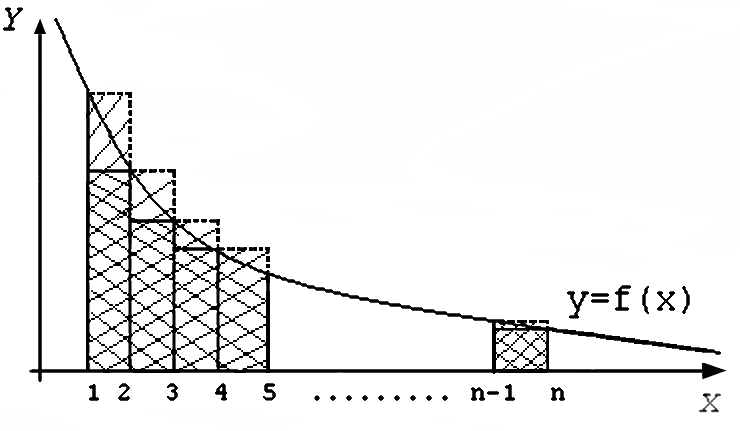
\includegraphics[width=6cm]{pics/25_1}
      \end{figure}
  \end{theorem}

  \begin{lemma}
      Если $f>0$, $f \in [a, \upomega] \rightarrow [0, +\infty)$, $f\in R[a,b]$ $\forall b \in (a, \upomega)$
      \\
      Тогда $\int\limits_a^\upomega f$ - сх $\lra$ $F(x) = \int\limits_a^x f$, $\e M < \infty:  F(x) \leqslant M $ $\forall x \in [a, \upomega)$
  \end{lemma}

  \begin{proof}
      ($\Rightarrow$) очевидно
      \\
      ($\Leftarrow$) почти очевидно, $f \geqslant 0 \Rightarrow F \nearrow$ и огр $\Rightarrow \e \lim\limits_{x \rightarrow \upomega} F(x) = \int\limits_a^\upomega f < +\infty$
  \end{proof}

  \begin{proof}
      $f(n+1) \leqslant \int\limits_n^{n+1} f \leqslant f(n)$ (видно через суммы Дарбу) $|\sum\limits_{n=1}^N$
      \\
      $\sum\limits_{n=1}^N f(n+1) \leqslant \int\limits_1^{N+1} f \leqslant \sum\limits_{n=1}^N f(n)$, при $N \rightarrow +\infty$ получим наше уравнение
      \\
      1) Если $\sum\limits_1^\infty f (n)$ - сх $\lra$ $\sum\limits_1^N f(n) \leqslant A \in \R \Rightarrow F(N+1) = \int\limits_1^{N+1} f \leqslant A \in \R$ сх
      \\
      2) Если $\int\limits_1^\infty f$ - сх $\Rightarrow \sum\limits_1^N f(n+1) \leqslant \int\limits_1^{N+1} f \leqslant \int\limits_1^\infty f \in \R$ - огр $\Rightarrow \sum\limits_1^N f(n+1)$ сх
  \end{proof}

  \begin{examples}
      \begin{enumerate}
          \item $\sum\limits_{n=1}^\infty \frac{1}{n^2}$. Рассмотрим $\int\limits_1^\infty \frac{1}{x^2} = - \frac{1}{x} |_1^\infty = 0 - (-1)$ - сх
          \item $\sum\limits_{n=1}^\infty \frac{1}{n^\upalpha}$. Сх. при $\upalpha > 1$, расх. при $\upalpha \leqslant 1$ (аналогично интегралу $\int\limits_{1}^\infty \frac{1}{x^\upalpha}$)
      \end{enumerate}
  \end{examples}

  \newpage
  \section{Признаки сравнения для несобственных интегралов.}

  \begin{Theorem}[\RNumb{1} признак сравнения]
      \[f,g: [a, \upomega) \rightarrow \R,\q f,g \geqslant 0,\q f,g \in R[a,b],\q b \in (a, \upomega),\]
      \[0 \leqslant f(x) \leqslant g(x)\q \forall x \in [a, \upomega)\]
      Тогда $\int\limits_a^\infty g$ - сх $\Rightarrow$ $\int\limits_a^\upomega f$ - сх ($\int\limits_a^\upomega f$ - расх $\Rightarrow$ $\int\limits_a^\infty g$ - расх)
  \end{Theorem}

  \begin{Proof}
      \[F(b) := \int\limits_a^b f \leqslant \int\limits_a^b g \leqslant \int\limits_a^\upomega g \in \R\]
      То есть $\int\limits_a^\upomega f$ - сх, т.к. $F \nearrow$ и огр сверху на $[a, \upomega)$
  \end{Proof}

  \begin{Theorem}[\RNumb{2} признак сравнения]
      \[f, g: [a, \upomega) \rightarrow (0, +\infty)$, $f,g \in R[a,b]$ $\forall b \in (a, \upomega)\]
      Тогда если $\e \lim\limits_{x \rightarrow \upomega_-} \dfrac{f(x)}{g(x)} \in (0, +\infty)$, то $\int\limits_a^\upomega f$ и $\int\limits_a^\upomega g$ - сх или расх одновременно
  \end{Theorem}

  \begin{Proof}
      \[k:=\lim\limits_{x \rightarrow \upomega_-} \frac{f(x)}{g(x)} \in (0, +\infty)$, $\E := \dfrac{k}{2}\]
      \[\Rightarrow \e b \in (a, \upomega): \forall x \in (b, \upomega)\ |\frac{f(x)}{g(x)} - k| < \E \Rightarrow  \E < \frac{f(x)}{g(x)} <  3\E\]
      То есть с некоторого места $f(x) \leqslant g(x)$, а так как $\int\limits_a^\upomega = \int\limits_a^b + \int\limits_b^\upomega$ и $\int\limits_a^b f, \int\limits_a^b g$ - конечные числа, то $\int\limits_a^\upomega f$ и $\int\limits_a^\upomega g$ - сх или расх одновременно по первому признаку
  \end{Proof}

  \begin{Example}
      \[\int\limits_0^{+\infty} e^{-x^2} dx= \int\limits_0^1 + \int\limits_1^{+\infty}\]
      \begin{figure}[H]
          \centering
          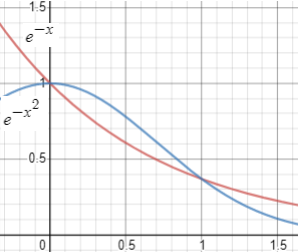
\includegraphics[width=4cm]{pics/26_1}
      \end{figure}
      \[e^{-x^2} \geqslant e^{-x} \Rightarrow x \in [0,1],\q \int\limits_0^1 e^{-x} = \frac{1}{e} \underset{\text{по \RNumb{1} пр. ср.}}{\Rightarrow} \int\limits_1^{+\infty} e^{-x^2}\text{ - сх}\]
  \end{Example}

  \begin{Example}
      \[\int\limits_1^{+\infty} \sin^2 \frac{1}{x} dx\]
      \[\lim\limits_{x\rightarrow\infty} \frac{\sin^2 \frac{1}{x}}{\frac{1}{x^2}} = 1 \in (0,+\infty) \Rightarrow \int\limits_1^{+\infty} \sin^2 \frac{1}{x} dx \text{ и } \int\limits_1^{+\infty} \frac{1}{x^2} dx \text{ - сх или расх одновр $\Rightarrow$ сх}\]
  \end{Example}

  \newpage
  \section{Абсолютная и условная сходимость интегралов. Сходимость следует из абсолютной сходимости.}
  \hypertarget{q27}{}

  \begin{definition}
      $f: [a, \upomega) \rightarrow \R$, $f \in R[a,b]$ $\forall b \in (a, \upomega)$

      $\int\limits_a^\upomega f$ - сх абсолютно $\lra$ $\int\limits_a^\upomega |f|$ - сх

      $\int\limits_a^\upomega f$ - сх условно $\lra$ $\int\limits_a^\upomega f$ - сх, $\int\limits_a^\upomega |f|$ - расх
  \end{definition}

  \begin{utv}
      $\int\limits_a^\upomega f$ - сх абсолютно $\Rightarrow$ сходится
  \end{utv}

  \begin{proof}
      Пусть $\int\limits_a^\upomega |f|$ - сх $\lra$ (кр. Больцано-Коши) $\forall \E > 0$ $\e A \in (a, \upomega): \forall b_1, b_2 \in (A, \upomega)$ $|\int\limits_{b_1}^{b_2} |f|| < \E \Rightarrow $ т.к. $|\int\limits_{b_1}^{b_2} f| \leqslant |\int\limits_{b_1}^{b_2} |f|| < \E$, то по кр. Б-К $\int\limits_{b_1}^{b_2} f$ - сх
  \end{proof}

  \begin{Example}
      \[\int\limits_0^{+\infty} \cos (x^3) dx = \begin{vmatrix}
        x^3 = t\\
        x = \sqrt[3]{t}
      \end{vmatrix} = \frac{1}{3} \int\limits_0^\infty \cos t \frac{dt}{t^{\frac{2}{3}}} = \frac{1}{3} \frac{\sin t}{t^{\frac{2}{3}}}\Big|_0^\infty + \frac{2}{9} \int\limits_0^\infty \frac{\sin t}{t^{\frac{5}{3}}} = \frac{2}{9} \int\limits_0^\infty \frac{\sin t}{t^{\frac{5}{3}}}\]
      \[\text{Исследуем }\int\limits_0^\infty \frac{|\sin t|}{t^{\frac{5}{3}}} = \int\limits_0^1 \frac{|\sin t|}{t^{\frac{5}{3}}} + \int\limits_1^\infty \frac{|\sin t|}{t^{\frac{5}{3}}}:\]
      \[\text{a) }\int\limits_0^1 \frac{|\sin t|}{t^{\frac{5}{3}}}$, $|sin t| \leqslant t\text{ на }[0,1]\]
      \[\int\limits_0^1 \frac{t}{t^{\frac{5}{3}}} = \int\limits_0^1 t^{-\frac{2}{3}} = 3t^{\frac{1}{3}} |_0^1 = 3\text{ - сх} \underset{\text{по \RNumb{1} пр ср}}{\Rightarrow} \int\limits_0^1 \frac{|\sin t|}{t^{\frac{5}{3}}}\text{ - cх}\]
      \[\text{б) }\int\limits_1^\infty \frac{|\sin t|}{t^{\frac{5}{3}}},\q \frac{|\sin t|}{t^{\frac{5}{3}}} \leqslant \frac{1}{t^{\frac{5}{3}}}\]
      \[\int\limits_1^\infty \frac{1}{t^{\frac{5}{3}}} = -\frac{3}{2} t^{-\frac{2}{3}} |_1^\infty = \frac{3}{2}\text{ - сх} \underset{\text{по \RNumb{1} пр ср}}{\Rightarrow} \int\limits_1^\infty \frac{|\sin t|}{t^{\frac{5}{3}}}\text{ - cх}\]
      \[\text{Значит }\int\limits_0^\infty \frac{\sin t}{t^{\frac{5}{3}}}\text{ - абс сх }\Rightarrow \int\limits_0^{+\infty} \cos (x^3) \text{ - сх}\]
  \end{Example}

  \newpage
  \section{Абсолютная и условная сходимость. Пример: $\int\limits_0^\infty \frac{\sin x}{x}$}

  Определения и теорему см. в билете \hyperlink{q27}{27}
  \begin{Example}
      \[\int\limits_0^\infty \frac{\sin x}{x} = \int\limits_0^{\frac{\pi}{2}} \frac{\sin x}{x} +  \int\limits_{\frac{\pi}{2}}^\infty \frac{\sin x}{x}\]
      \[1)\q \int\limits_{\frac{\pi}{2}}^\infty \frac{\sin x}{x} = \frac{-\cos x}{x} \Big|_\frac{\pi}{2}^\infty - \int\limits_\frac{\pi}{2}^\infty \frac{\cos x}{x^2} = \int\limits_\frac{\pi}{2}^\infty \frac{\cos x}{x^2}\]
      \[\text{Исследуем }\int\limits_\frac{\pi}{2}^\infty \frac{\cos x}{x^2}\text{ на абс сходимость}.\q \frac{|\cos x|}{x^2} \leqslant \frac{1}{x^2}, \text{ а} \int\limits_\frac{\pi}{2}^\infty \frac{1}{x^2}\text{ - сходится}\]
      \[\Rightarrow \text{ по 1 признаку сравнения } \int\limits_\frac{\pi}{2}^\infty \frac{|\cos x|}{x^2}\text{ - сх }\Rightarrow \int\limits_\frac{\pi}{2}^\infty \frac{\cos x}{x^2}\text{ - сх абс }\Rightarrow \int\limits_{\frac{\pi}{2}}^\infty \frac{\sin x}{x}\text{ - сх}\]
      \[2)\q \int\limits_0^{\frac{\pi}{2}} \frac{|\sin x|}{x}\]
      \[\text{Знаем, что }\lim\limits_{x \rightarrow 0} \frac{|\sin x|}{x} = 1.\text{ Кроме того, }\frac{|\sin x|}{x} < 1,\text{ значит на конечном}\]
      \[\text{промежутке }(0, \frac{\pi}{2}]\text{ интеграл конечный }\Rightarrow \int\limits_{0}^\infty \frac{\sin x}{x}\text{ - сх}\]
      \[\text{3) Покажем, что }\int\limits_{\frac{\pi}{2}}^\infty \frac{|\sin x|}{x}\text{ - расх. }\Rightarrow \int\limits_{0}^\infty \frac{|\sin x|}{x}\text{ - расх}\]
      \[|\sin x| \geqslant |\sin^2 x|,\q \int\limits_{\frac{\pi}{2}}^\infty \frac{\sin^2 x}{x} = \int\limits_{\frac{\pi}{2}}^\infty \frac{1 - \cos 2x}{x} = \frac{1}{2} \int\limits_{\frac{\pi}{2}}^\infty \frac{dx}{x}\text{(расх)} + \int\limits_{\frac{\pi}{2}}^\infty \frac{\cos 2x}{x}\text{(сх)}\]
  \end{Example}

  \newpage
  \section{Признаки Дирихле и Абеля для несобственных интегралов (док-во одного из них).}

  \begin{Theorem} [признак Абеля-Дирихле]
      \[f,g: [a, \upomega) \rightarrow \R,\q f \in C[a,\upomega),\q g \in C^1 [a,\upomega),\text{ g - монотонна.}\]
      Тогда если выполнено одно из условий:
      \[\text{(A) }\int_a^\upomega \text{f - сх, g - огр}\]
      \[\text{(Д) }F(x) := \int\limits_a^x \text{f - огр, }g(x) \underset{x \rightarrow \upomega_-}{\rightarrow} 0\]
      Тогда $\int\limits_a^\upomega f g$ - сх
  \end{Theorem}

  \begin{proof}
      (Д) без теоремы Бонне
      \[|F(x)| \leqslant C: g(x) \underset{x \rightarrow \upomega_-}{\rightarrow} 0\]
      \[\lim\limits_{b \rightarrow \upomega_-} \int\limits_a^b f g = \lim\limits_{b \rightarrow \upomega_-} (F g |_a^b - \int\limits_a^b F g') = F(a) g(a) - \lim\limits_{b \rightarrow \upomega_-} \int\limits_a^b F g'\]
      Исследуем интеграл на абс сходимость.
      \[\int\limits_a^b |F g'| \leqslant C \int\limits_a^b |g'| = \text{(т.к. g - монотонна)} C |\int\limits_a^b g'| = C |g(b) - g(a)| \underset{b \rightarrow \upomega_-}{\rightarrow} C |g(a)|\]
      Таким образом инт. ограничен $\Rightarrow$ изначальный сходится
  \end{proof}

  \newpage
  \section{Признаки Дирихле и Абеля для рядов (док-во одного из них).}

  \begin{definition}
      $A_n := \sum\limits_{k=1}^n a_k$, $A_0=0$
  \end{definition}

  \begin{Theorem} [преобразование Абеля]
      \[\sum\limits_{k=1}^n a_k b_k = A_n b_n + \sum\limits_{k=1}^{n-1} A_k (b_k - b_{k+1})\]
  \end{Theorem}

  \begin{Proof}
      \begin{multline*}
          $$\sum\limits_{k=1}^n a_k b_k = \sum\limits_{k=1}^n (A_k - A_{k-1}) b_k = \sum\limits_{k=1}^n A_k b_k - \sum\limits_{k=1}^n A_{k-1} b_k =\\
          =\sum\limits_{k=1}^n A_k b_k - \sum\limits_{k=0}^{n-1} A_k b_{k+1} = A_n b_n + \sum\limits_{k=0}^{n-1} A_k (b_k - b_{k+1})$$
      \end{multline*}
  \end{Proof}

  \begin{theorem} [признак Дирихле для рядов]
      Пусть $A_n$ - огр., $b_k \rightarrow 0$, $b_k$ - монотонно. Тогда $\sum\limits_{k=1}^\infty a_k b_k$ - сх
  \end{theorem}

  \begin{proof}
      \[\sum\limits_{k=1}^n a_k b_k = A_n b_n + \sum\limits_{k=1}^{n-1} A_k (b_k - b_{k+1}) \underset{n \rightarrow \infty}{\rightarrow} \sum\limits_{k=1}^{n-1} A_k (b_k - b_{k+1})\]
      Ряд $\sum\limits_{k=1}^\infty a_k b_k$ - сх $\lra$ $\sum\limits_{k=1}^\infty A_k (b_k - b_{k+1})$ - сх $\lra$ все частичные суммы огр
      \\
      $\sum\limits_{k=1}^N |A_k| |b_k - b_{k+1}| \leqslant M \sum\limits_{k=1}^N |b_k - b_{k+1}| = M |b_1 - b_{N+1}| \leqslant 2 M |b_1| \Rightarrow$ исх ряд сх
  \end{proof}

  \begin{theorem} [признак Абеля для рядов]
      Пусть $A_n$ - сх. $b_k$ - монотонно, $b_k$ - огр. Тогда $\sum\limits_{k=1}^\infty a_k b_k$ - сх
  \end{theorem}
\end{document}
